\section*{Supplementary Material}

\subsection*{Per-Keypoint (Micro) PCK Results}
\label{sec:supp_micro}

Table~\ref{tab:micro_pck} reports per-keypoint (micro) PCK on the SPair-71k test split, complementing the per-image (macro) results in Table~\ref{tab:quantitative_results}. Micro PCK weights each keypoint equally regardless of how many annotated points an image contains, making it more sensitive to frequently occurring keypoints (e.g., eyes, wheels) than macro PCK.

\begin{table}[ht]
    \centering
    \caption{Per-keypoint (micro) PCK on the SPair-71k test split. WSA = Windowed Soft-Argmax; FT = Fine-Tuned last $N$ blocks (with photometric augmentation).}
    \label{tab:micro_pck}
    \resizebox{\columnwidth}{!}{%
    \begin{tabular}{llcccc}
        \toprule
        \textbf{Model} & \textbf{Method} & \textbf{Blocks} & \textbf{PCK@0.05} & \textbf{PCK@0.10} & \textbf{PCK@0.20} \\
        \midrule
        \multicolumn{6}{l}{\textit{Training-Free Baseline}} \\
        DINOv2 (ViT-B) & Baseline (Argmax) & — & 0.201 & 0.299 & 0.411 \\
        DINOv2 (ViT-B) & Baseline + WSA    & — & 0.205 & 0.301 & 0.413 \\
        DINOv3 (ViT-B) & Baseline (Argmax) & — & 0.236 & 0.355 & 0.475 \\
        DINOv3 (ViT-B) & Baseline + WSA    & — & 0.239 & 0.357 & 0.477 \\
        SAM    (ViT-B) & Baseline (Argmax) & — & 0.155 & 0.242 & 0.379 \\
        SAM    (ViT-B) & Baseline + WSA    & — & 0.155 & 0.242 & 0.380 \\
        \midrule
        \multicolumn{6}{l}{\textit{Light Fine-Tuning (last $N$ blocks)}} \\
        DINOv2 (ViT-B) & FT (Argmax) & 1 & 0.320 & 0.473 & 0.619 \\
        DINOv2 (ViT-B) & FT + WSA    & 1 & 0.333 & 0.479 & 0.622 \\
        DINOv2 (ViT-B) & FT (Argmax) & 2 & 0.292 & 0.485 & 0.656 \\
        DINOv2 (ViT-B) & FT + WSA    & 2 & 0.329 & \textbf{0.504} & \textbf{0.662} \\
        DINOv2 (ViT-B) & FT (Argmax) & 4 & 0.163 & 0.324 & 0.517 \\
        DINOv2 (ViT-B) & FT + WSA    & 4 & 0.207 & 0.352 & 0.529 \\
        DINOv3 (ViT-B) & FT (Argmax) & 1 & 0.343 & 0.520 & 0.661 \\
        DINOv3 (ViT-B) & FT + WSA    & 1 & 0.357 & 0.527 & 0.665 \\
        DINOv3 (ViT-B) & FT (Argmax) & 2 & 0.311 & 0.488 & 0.659 \\
        DINOv3 (ViT-B) & FT + WSA    & 2 & 0.345 & 0.505 & 0.665 \\
        DINOv3 (ViT-B) & FT (Argmax) & 4 & 0.215 & 0.385 & 0.567 \\
        DINOv3 (ViT-B) & FT + WSA    & 4 & 0.256 & 0.411 & 0.579 \\
        SAM    (ViT-B) & FT (Argmax) & 1 & 0.069 & 0.135 & 0.256 \\
        SAM    (ViT-B) & FT + WSA    & 1 & 0.073 & 0.138 & 0.257 \\
        SAM    (ViT-B) & FT (Argmax) & 2 & 0.062 & 0.115 & 0.215 \\
        SAM    (ViT-B) & FT + WSA    & 2 & 0.067 & 0.118 & 0.216 \\
        SAM    (ViT-B) & FT (Argmax) & 4 & 0.061 & 0.112 & 0.212 \\
        SAM    (ViT-B) & FT + WSA    & 4 & 0.066 & 0.115 & 0.214 \\
        \midrule
        \multicolumn{6}{l}{\textit{LoRA (rank 8, $\alpha{=}16$, last $N$ blocks)}} \\
        DINOv2 (ViT-B) & LoRA (Argmax) & 1 & 0.277 & 0.411 & 0.550 \\
        DINOv2 (ViT-B) & LoRA + WSA    & 1 & 0.287 & 0.415 & 0.553 \\
        DINOv2 (ViT-B) & LoRA (Argmax) & 2 & 0.291 & 0.438 & 0.587 \\
        DINOv2 (ViT-B) & LoRA + WSA    & 2 & 0.311 & 0.449 & 0.593 \\
        DINOv2 (ViT-B) & LoRA (Argmax) & 4 & 0.143 & 0.289 & 0.478 \\
        DINOv2 (ViT-B) & LoRA + WSA    & 4 & 0.170 & 0.312 & 0.489 \\
        DINOv3 (ViT-B) & LoRA (Argmax) & 1 & 0.300 & 0.452 & 0.599 \\
        DINOv3 (ViT-B) & LoRA + WSA    & 1 & 0.308 & 0.458 & 0.603 \\
        DINOv3 (ViT-B) & LoRA (Argmax) & 2 & 0.339 & 0.500 & 0.651 \\
        DINOv3 (ViT-B) & LoRA + WSA    & 2 & \textbf{0.357} & 0.511 & 0.656 \\
        DINOv3 (ViT-B) & LoRA (Argmax) & 4 & 0.173 & 0.332 & 0.518 \\
        DINOv3 (ViT-B) & LoRA + WSA    & 4 & 0.208 & 0.358 & 0.529 \\
        SAM    (ViT-B) & LoRA (Argmax) & 1 & 0.089 & 0.164 & 0.297 \\
        SAM    (ViT-B) & LoRA + WSA    & 1 & 0.092 & 0.167 & 0.298 \\
        SAM    (ViT-B) & LoRA (Argmax) & 2 & 0.041 & 0.086 & 0.178 \\
        SAM    (ViT-B) & LoRA + WSA    & 2 & 0.046 & 0.089 & 0.181 \\
        SAM    (ViT-B) & LoRA (Argmax) & 4 & 0.046 & 0.090 & 0.183 \\
        SAM    (ViT-B) & LoRA + WSA    & 4 & 0.048 & 0.093 & 0.186 \\
        \bottomrule
    \end{tabular}
    }
\end{table}

\subsection*{Per-Category PCK Results}
\label{sec:supp_category}

Figure~\ref{fig:per_category_supp} shows PCK@0.10 broken down by SPair-71k object category for all configurations. Rigid, texturally distinctive categories (bus, bottle, car, aeroplane) achieve the highest correspondence accuracy. Articulated or texture-poor categories (person, horse, cow) are consistently harder across all backbones and adaptation strategies. The category ranking is stable across methods, confirming that category difficulty is driven primarily by intrinsic shape variability rather than the choice of backbone or adaptation strategy.

\begin{figure}[ht]
    \centering
    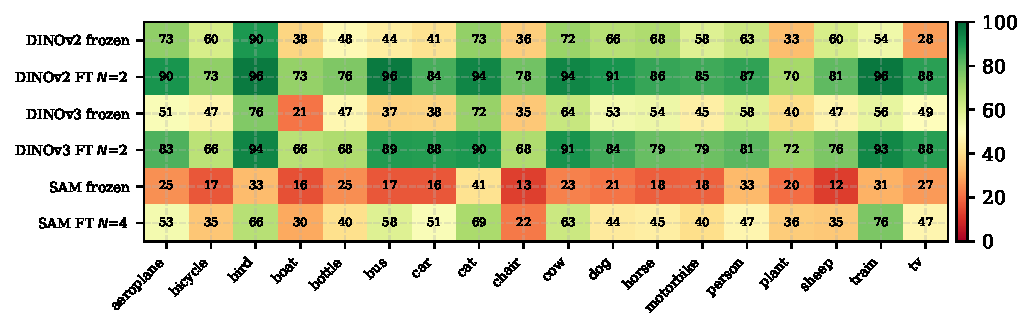
\includegraphics[width=\columnwidth]{img/per_category_a0.pdf}
    \caption{Per-category PCK@0.10 heatmap for all configurations. Rigid categories (bus, bottle, car) achieve higher accuracy; articulated categories (person, horse, cow) are harder across all methods.}
    \label{fig:per_category_supp}
\end{figure}

\subsection*{GitHub Repository}
\label{sec:repo}

\url{https://github.com/lucaosti/Semantic-Correspondence}
